\documentclass{article}
\usepackage{amsmath}
\usepackage{algorithm}  
\usepackage{algorithmic}
\usepackage{listings}
\usepackage{graphicx}
\usepackage{latexsym}
\usepackage{geometry}
\geometry{left=2.5cm,right=2.5cm,top=2.5cm,bottom=2.5cm}
\begin{document}

\title{CS143 Project 2 Part B}
\author{Yao Xie 804946717 allenxie@cs.ucla.edu\\Kaiyuan Xu 505033984 kyxu@g.ucla.edu}
\maketitle

\textbf{1.}
\begin{figure}[H]
\centering
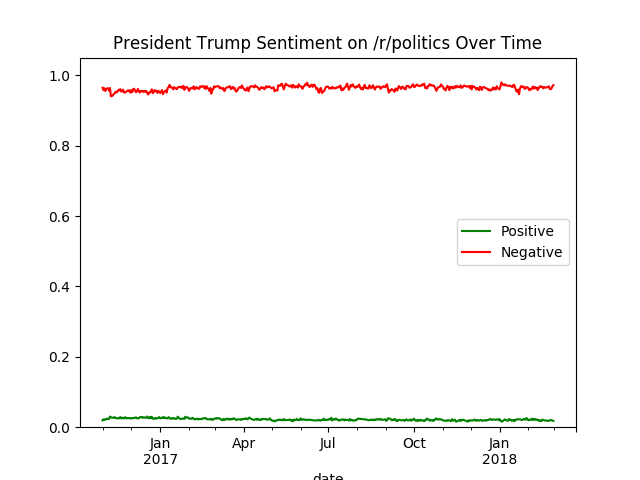
\includegraphics[width=0.7\textwidth]{1.png}
\caption{Sentiment over time}\label{1}
\end{figure}


\textbf{2.} Parameters $vmin$ and $vmax$ has been adjusted.
\begin{figure}[H]
\centering
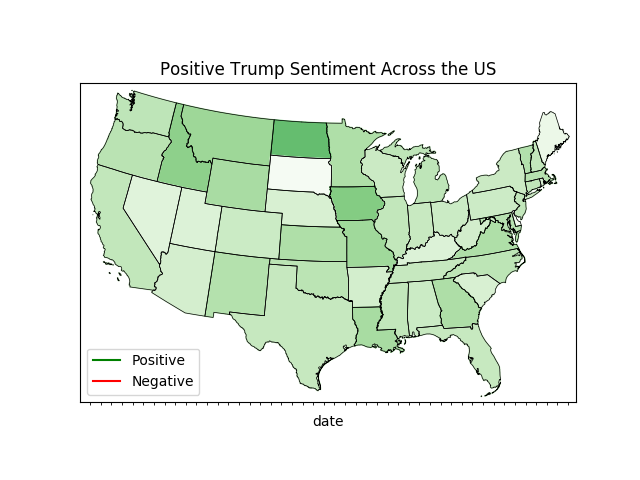
\includegraphics[width=0.7\textwidth]{2.png}
\caption{Positive across the US}\label{2}
\end{figure}
\begin{figure}[H]
\centering
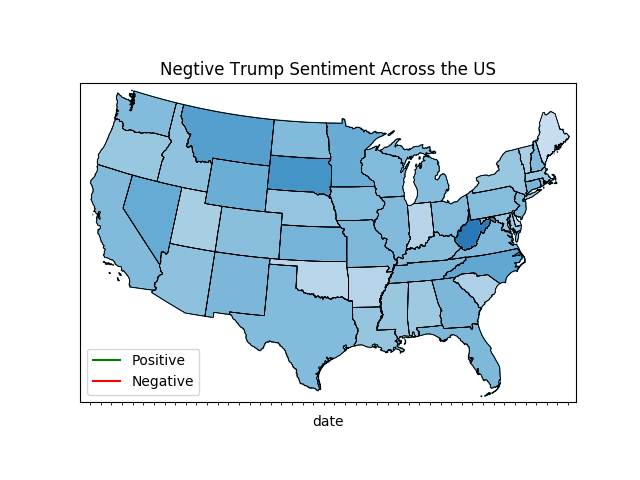
\includegraphics[width=0.7\textwidth]{3.png}
\caption{Negative across the US}\label{3}
\end{figure}


\textbf{3.}
\begin{figure}[H]
\centering
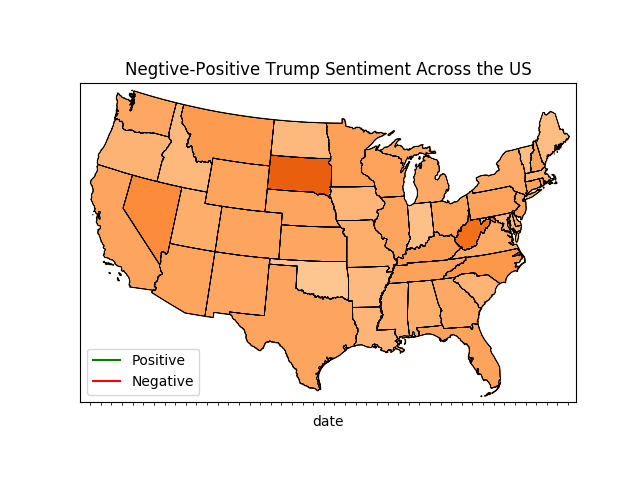
\includegraphics[width=0.7\textwidth]{4.png}
\caption{Negative-Positive across the US}\label{4}
\end{figure}

\textbf{4.}
\begin{figure}[H]
\centering
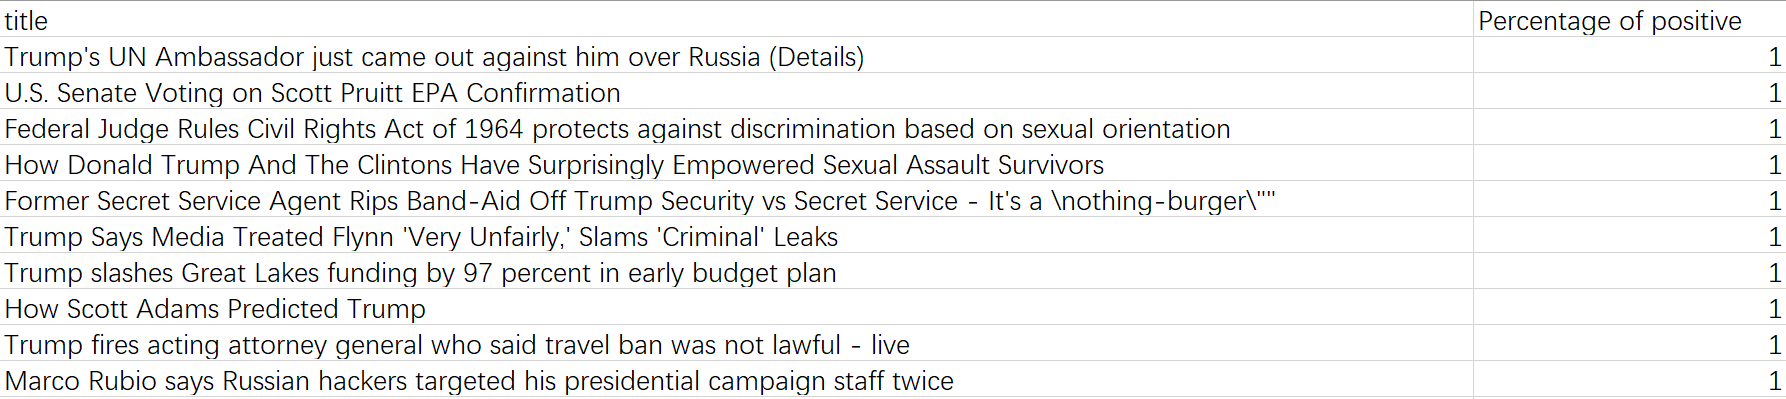
\includegraphics[width=\textwidth]{10.png}
\caption{Positive story}\label{5}
\end{figure}
\begin{figure}[H]
\centering
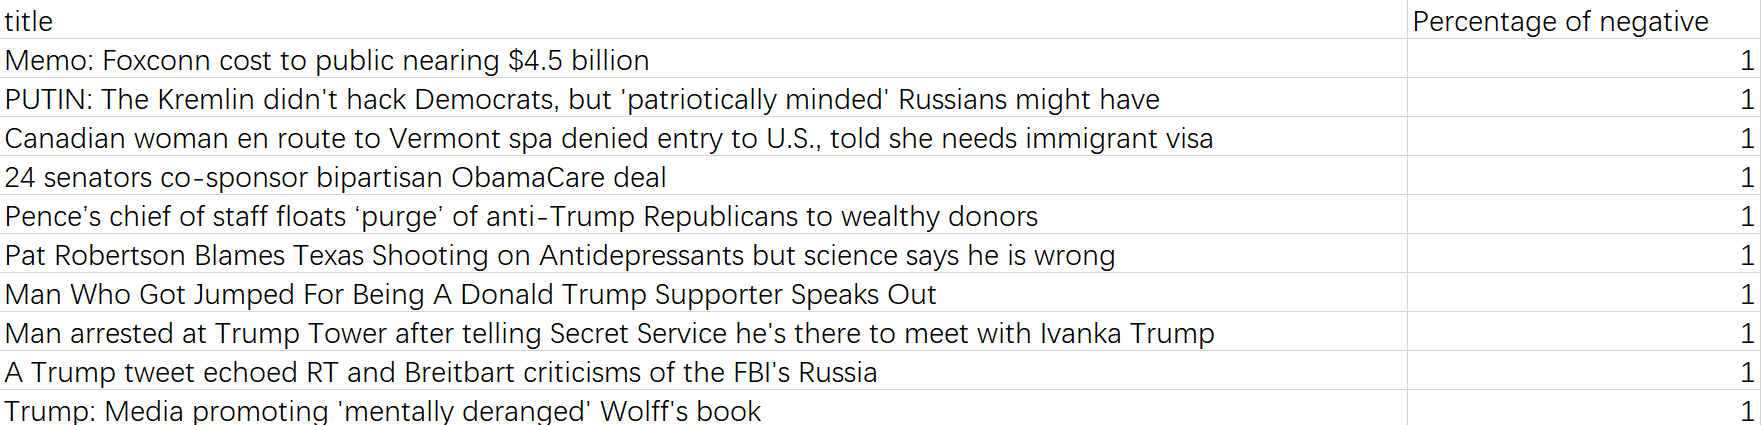
\includegraphics[width=\textwidth]{11.png}
\caption{Negative story}\label{6}
\end{figure}

\textbf{5.}
\begin{figure}[H]
\centering
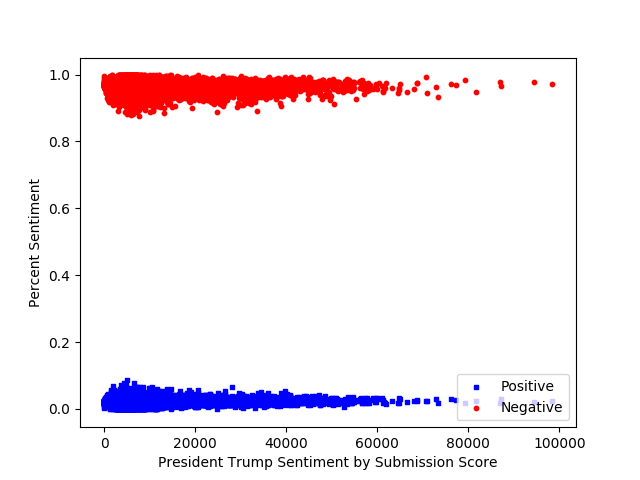
\includegraphics[width=0.7\textwidth]{5.png}
\caption{Sentiment by submission score}\label{7}
\end{figure}
\begin{figure}[H]
\centering
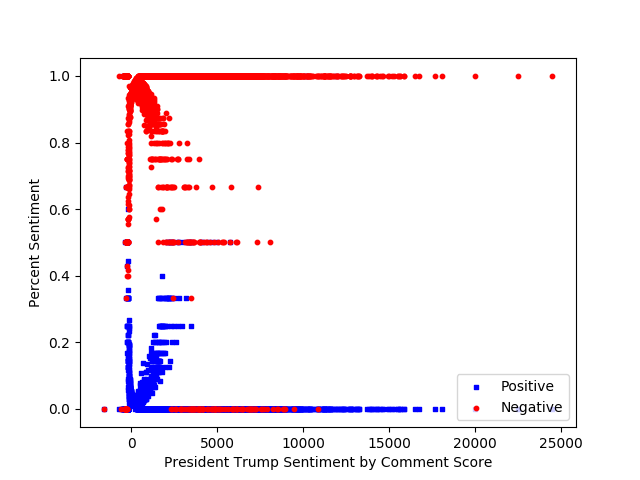
\includegraphics[width=0.7\textwidth]{6.png}
\caption{Sentiment by comment score}\label{8}
\end{figure}


\textbf{7.} The AUC for negative results is 0.94 and the AUC for positive results is 0.93. From the curve, we can see that the trained model is fairly good.
\begin{figure}[H]
\centering
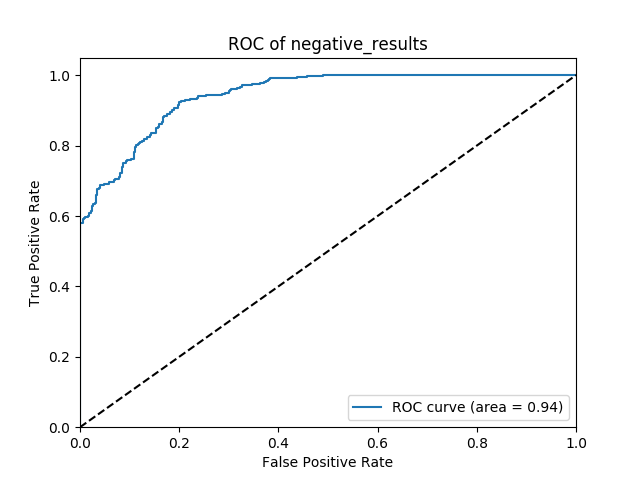
\includegraphics[width=0.7\textwidth]{8.png}
\caption{Negative ROC}\label{9}
\end{figure}
\begin{figure}[H]
\centering
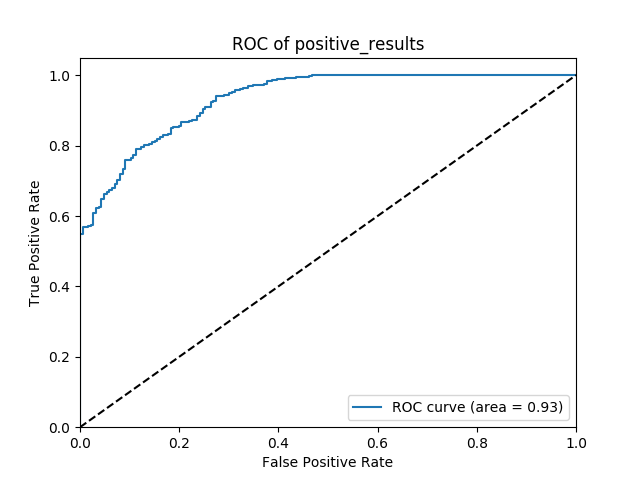
\includegraphics[width=0.7\textwidth]{9.png}
\caption{Positive ROC}\label{10}
\end{figure}


\textbf{8.}\\

We can see from Figure~\ref{1} that negative comments are significantly more than positive comments. The possible reasons may be that this dataset is biased and /r/politics thinks about President Trump negatively. We can see from Figure~\ref{2} and~\ref{3} that it varies by state, and from Figure~\ref{4} that, the deeper the color is, the more negatively /r/politics thinks about President Trump. From Figure~\ref{1} again, we can see that it does not really vary over time, the sentiment is roughly stable. And from Figure~\ref{5} and~\ref{6}, we can see it varies by story, different stories have different sentiments. We can see from Figure~\ref{7} and~\ref{8} that submission score might be a good feature for classificaition, and comment score could probably not be a good feature for classification.\\


\textbf{QUESTION 1.}\\

The functional dependencies in label dataset could be:
\begin{center}
$input\_id \rightarrow \{labeldem, labelgop, labeldjt\}$.
\end{center}
\hfill

\textbf{QUESTION 2.}\\

It doesn't look normalized. The existence of columns $\{subreddit, subreddit\_id, subreddit\_type\}$ is redundant since we need to ensure the dependency between $subreddit\_id$ and $subreddit, subreddit\_type$ when inserting/updating. We can decompose the whole table as $R_1 = \{\underline{subreddit\_id}, subreddit, subreddit\_type\}$ with $R_2 = \{\text{all columns without }'subreddit'\text{ and }'subreddit\_type' \}$. But by doing so, there may be a foreign key set on 'subreddit\_id' and this may cause insert/update integrity. And this can avoid a big join when querying. So maybe that's why the collector stored the data in a whole table.\\

\textbf{QUESTION 3.}\\

Figure~\ref{q32} is part of the codes to generate the join result. And Figure~\ref{q31} shows the results of join between label and comments in task 3 with explain() and the corresponding output. 

And we noticed that the procedure of a inner join here can be separated into three parts: first of all, Spark load the tables to be joined with filtering the invalid rows with null value of the attributes as the join key; then it will select the corresponding attributes from each table according to the select schema, and this part is similar to do select operation before the join operation which may save space and time when joining; finally Spark did a hash-join on the join keys as well as a selection again just to match the final result.
\begin{figure}[H]
\centering
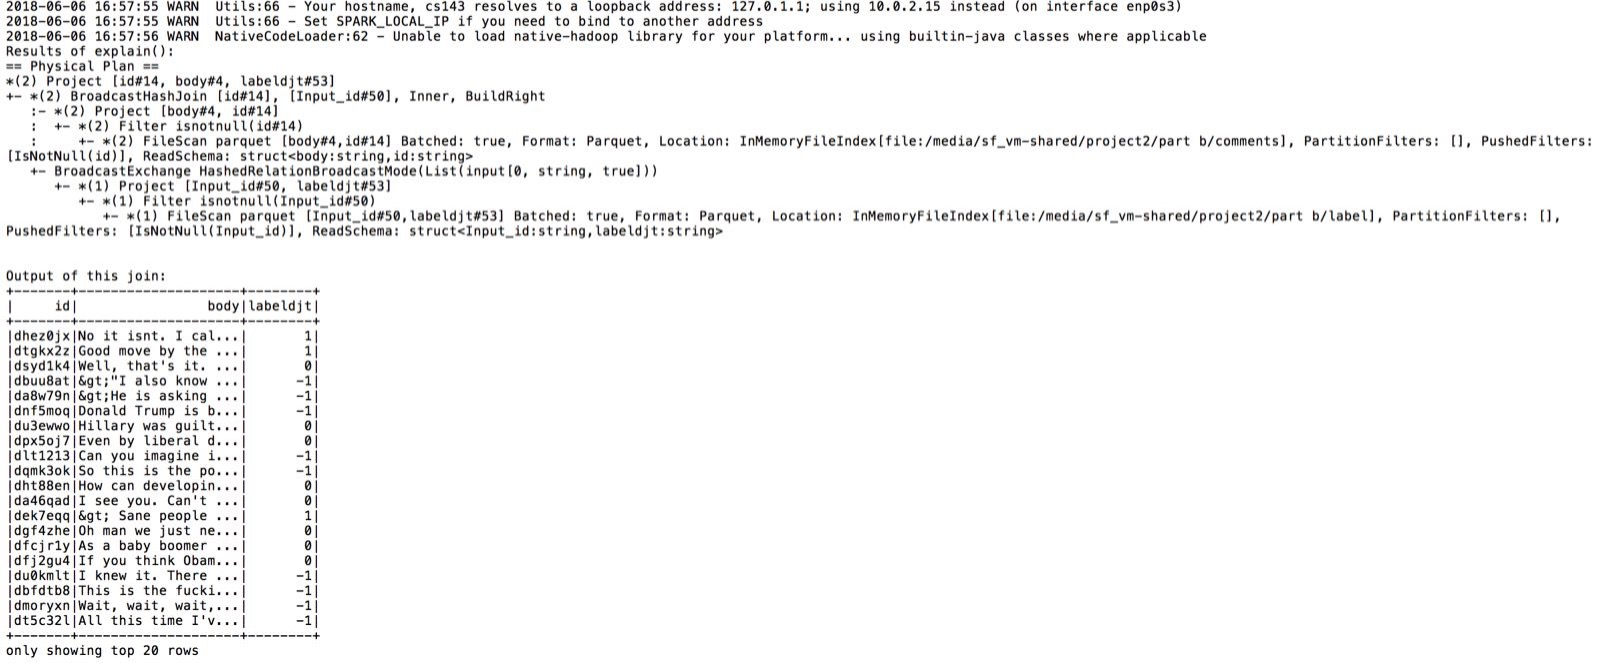
\includegraphics[width=\textwidth]{q3-1.jpg}
\caption{Result of explain join and the output}\label{q31}
\end{figure}

\begin{figure}[H]
\centering
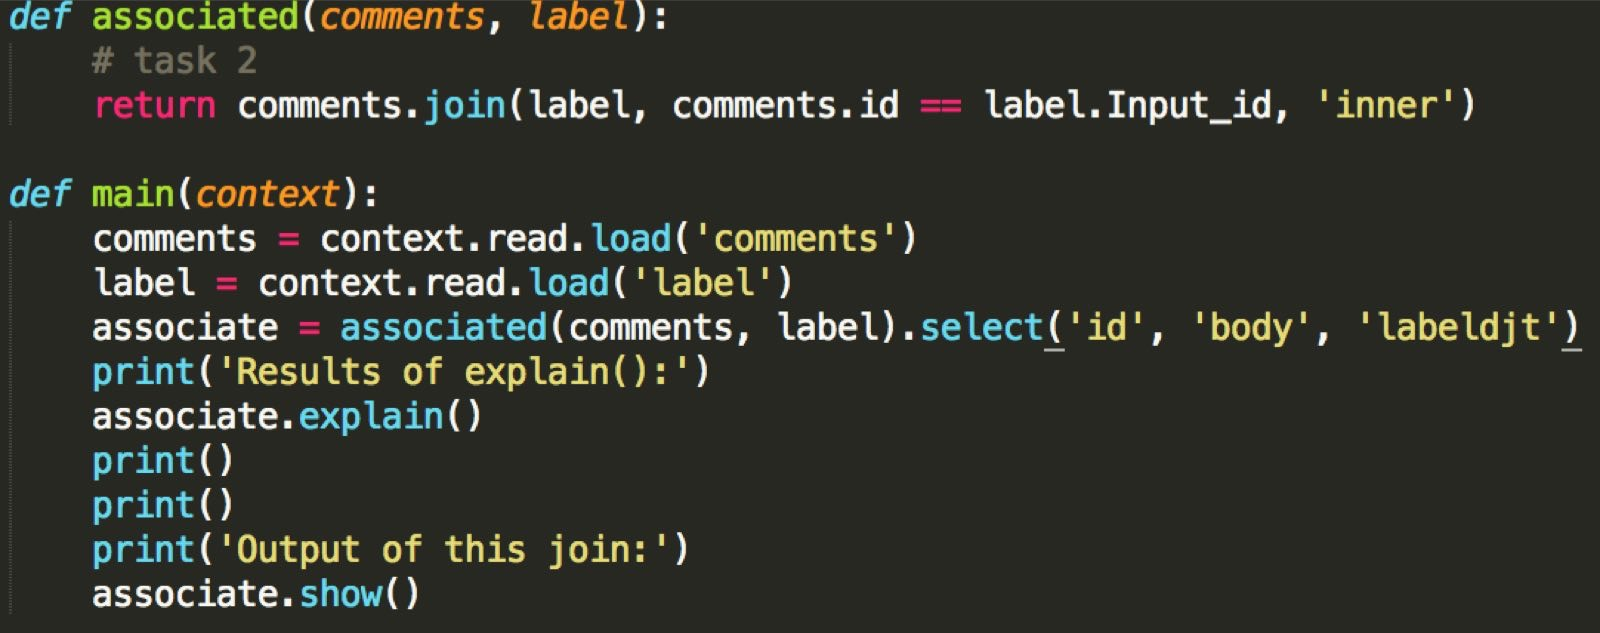
\includegraphics[width=\textwidth]{q3-2.jpg}
\caption{Part of the codes to do explain}\label{q32}
\end{figure}


\end{document}
